75. \begin{figure}[ht!]
\center{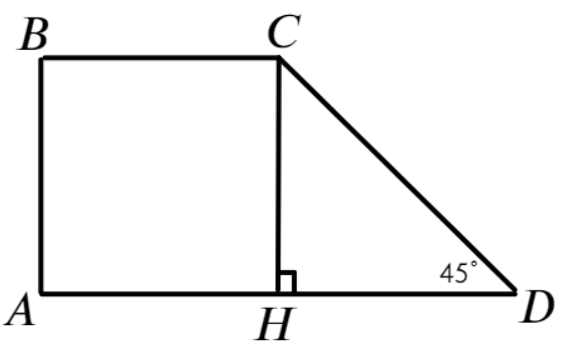
\includegraphics[scale=0.35]{g8-74.png}}
\end{figure}\\
Проведём высоту $CH.$ Тогда $ABCH$ является прямоугольником, а так как $AB=BC,$ то и квадратом. Так как $\angle D=45^\circ,\ \angle HCD=90^\circ-45^\circ=45^\circ$ и треугольник $CHD$ является равнобедренным, $HD=CH=BC=AB.$ Пусть $BC=x,$ тогда $S_{ABCD}=\cfrac{1}{2}\cdot{x}\cdot(x+x+x)=\cfrac{3}{2}x^2=24,\ x^2=16,\ x=4$см.\\
